\documentclass[preprint,3p]{elsarticle}
%\documentclass[preprint]{aastex}
\usepackage{aas_macros}
\usepackage{amsmath,amssymb}
\usepackage{mathrsfs}
\usepackage{graphicx}
\usepackage{bm}
\usepackage{hyperref}
\DeclareMathOperator\erf{erf}
\newcommand{\mli}[1]{\mathit{#1}}
%\usepackage{epstopdf}


\begin{document}

%\begin{frontmatter}
%
%\title{Toy Model}
%\author{A.~G. Kim\corref{cor1}}
%\ead{agkim@lbl.gov}
%\address{Physics Division, Lawrence Berkeley National Laboratory, 1 Cyclotron Road, Berkeley CA, USA 94720}
%
%\begin{abstract}
%\end{abstract}
%\begin{keyword}
%\end{keyword}
%\end{frontmatter}

\section{Likelihood and Posterior}
\label{likelihood:sec}

The ambition is to construct a model to determine the likelihood of DES-like
supernova data. 
The conceptual structure of the model is shown in Figure~\ref{pgm:fig}. 
\begin{figure}[htbp] %  figure placement: here, top, bottom, or page
   \centering
   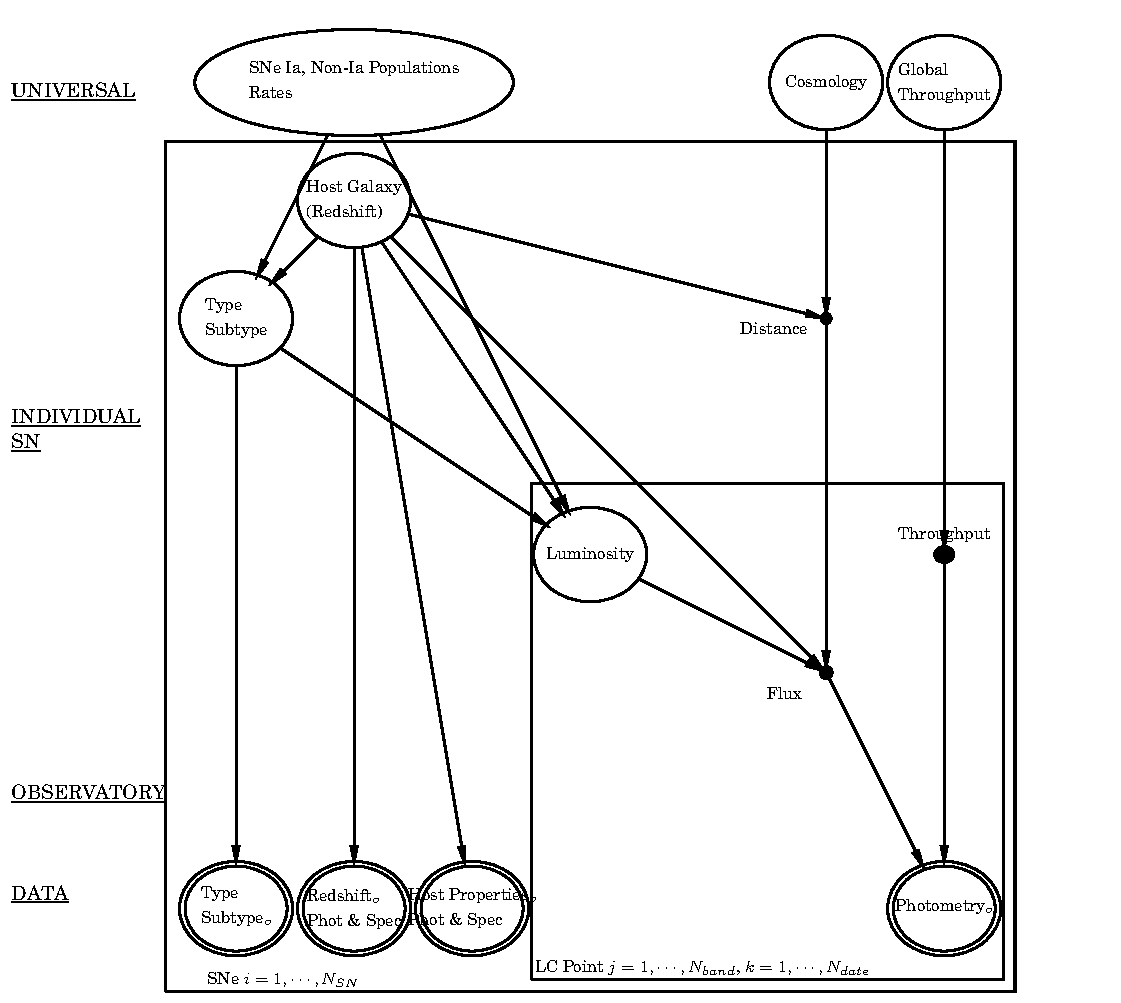
\includegraphics[width=6.5in]{../results//hdpgm.pdf} 
   \caption{Probabilistic Graphical Model for the SN~Ia analysis.  
   \label{pgm:fig}}
\end{figure}

The model has the following types of observables $O$ that
may be observed for each supernova:
\begin{itemize}
\item $c$: Counts of the photometric measurements (light curves).
\item $s$: Counts of the spectroscopic measurements.
\item $z$: Redshift.
\item $T$: Transient type.
\end{itemize}
The measurements made of the observables are labeled  with a subscript ``o''.

There are top-level  sets of parameters $M$ that correspond to photometric calibration, cosmology,
host-galaxy properties, and transient properties.
There are two sets of intermediary parameters $M_I$ that correspond to luminosity $L$ and type $\tau$.

The model describes transients and their observables.  We are particularly interested in the pdf of those observables
given the model.  The pdf is dependent on the sample and we consider two such samples: an underlying sample
that represents the distribution of all possible transients and observables accommodated by the model; and
an analysis sample that represents the distribution of transients and observables that end up being analyzed.
The analysis sample differs from the underlying sample in that the transients of the former 
must be discovered, pass photometric selection criteria, and for the SN~Ia sample be selected for spectroscopic
observation, have a successful type from the spectrum, and be typed as SN~Ia.
The pdf of the underlying sample is denoted as $p(O|M,M_I)$ whereas the pdf of the analysis sample, the likelihood,
is denoted $\mathcal{L}_S(O | M, M_I)$. 
The two are related by
\begin{align}
% \mathcal{L}_S(O_o | M, M_I) & = \frac{\epsilon(O_o, M, M_I) p(O_o|M, M_I)}{\int  \epsilon(O, M, M_I) p(O|M, M_I)dO},
\mathcal{L}(O_o | M, M_I) & = \frac{p_S(O_o|M, M_I)}{\int  p_S(O|M, M_I)dO},
\label{likelihood:eqn}
\end{align}
where
\begin{align}
p_S(O|M, M_I) &= p(O, disc=True, anal=True, sobs=True, type=True, T=SNIa |M, M_I).
\end{align}

As the sample-inclusion probabilities and the uncertainties in $O_o$ are expected to be uncorrelated between different transients
 the likelihood can be split into contributions
from each,
\begin{align*}
\mathcal{L}(O_o | M, M_I) & = \frac{\prod_{\alpha \in transients} p_S(O_o^\alpha|M, M_I)}{\prod_{\alpha \in transients} \int  p_S(O^\alpha|M, M_I)dO^\alpha}.
\end{align*}
Note that we work with counts:  correlated calibration uncertainties would prevent this splitting for fluxes.


We now consider the terms in the likelihood contributed by each transient and omit the $\alpha$ superscript. 
The dependencies of the parameters are charted through the PGM to give for transients with a  spectroscopic type measurement
\begin{align*}
p(O| M, M_I) & = P(T |\tau) p(z | M) p(c | L, M) p (s|L, M),
\end{align*}
and for transients without a type measurement (not relevant for the SN~Ia-only analysis but included for completeness)
\begin{align*}
p(O| M, M_I) & = p(z | M) p(c | L, M),
\end{align*}
where the photometric and spectroscopic observations have independent measurement uncertainties.

The probability density for an object to enter the analysis sample can be broken out
\begin{align}
p_S(O|M, M_I) &= p(O, disc=True, anal=True, sobs=True, type=True, T=SNIa |M, M_I)\\
&= P(T, T=SNIa| s, c, disc=True, anal=True, sobs=True, type=True, M, M_I)\\
& \times  p(s, type=True | c, disc=True, anal=True, sobs=True, M, M_I)\\
& \times  p(c, disc=True, anal=True, sobs=True| M, M_I)\\
&= P(T, T=SNIa| M, M_I)  p(s, type=True | M, M_I) \\
& \times  p(c, disc=True, anal=True, sobs=True| M, M_I).
\end{align}

%Transient discovery and sample selection are purely based on observed photometry $c$.
%The decision for spectroscopic follow-up is also based on observed photometry,  though perhaps external redshift estimates
%of the possible host galaxy may come into play.  The success of the typing measurement should primarily depend
%on the signal $s$, but may also depend on the type and host properties. 

A frequentist analysis can proceed with this likelihood.
Alternatively, the Bayesian posterior is specified by parameter priors as follows:
\begin{align*}
p(M, M_i | O_o) & \propto \mathcal{L}(O_o| M, M_I) p(M_I|M) p(M)\\
 & \propto \mathcal{L}(O_o| M, M_I) p(L| \tau, M) p(\tau|M) p(M).
\end{align*}
Once all the $p$'s and $P$'s are specified we are ready to analyze!

\section{Probabilities: Minding Ones P's and p's}
Section~\ref{likelihood:sec} introduces the probabilities and probability distribution functions that describe the likelihood
and posterior for the model shown in Figure~\ref{pgm:fig}.
In this Section we present one possible model by specifying those probabilities; the assembly of other models should
resemble this example.

\subsection{$p(M)$: Priors on the Top-Level Parameters}
\begin{itemize}
\item
Flat $w$CDM cosmological parameters are drawn from top-hat distributions
\begin{align}
\Omega_M & \sim  {\mathcal{U}}(0,1)\\
w_0 & \sim \mathcal{U}(-1.5, -0.1).
\end{align}

\item
Photometric zeropoints for each band are given by
\begin{equation}
Z \sim \mathcal{N}\left(0,\left(\frac{\ln{10}}{2.5}\right)^2 C_{cal}\right),
\end{equation}
where $C_{cal}$ is the covariance of the calibration zeropoints calculated by Chris Lidman.
(The PGM anticipates a more complicated calibration approach.)

\item
There are a number of parameters that describe the supernova populations.

The luminosity of SNe~Ia as a function of time and wavelength is described by the SALT2 model and
the linear relation of its parameters with absolute magnitude.
The following priors are taken from the Rubin et al.\ UNITY paper:
\begin{align}
M_{SNIa} & \sim \mathcal{U}(-20, -18) \\
\arctan{\alpha_{SNIa}} & \sim \mathcal{U}(-0.2, 0.3) \\
\arctan{\beta_{SNIa}} & \sim \mathcal{U}(-1.4, 1.4),
\end{align}
and for ``hyperparameters'' that describe the distributions of the per-supernova parameters
\begin{align}
\log_{10}{R^{x_0}_{SNIa}} & \sim \mathcal{U}({-2}, {-0.5})\\
\log_{10}{R^{x_1}_{SNIa}} & \sim \mathcal{U}({-0.5}, {0.5})\\
\log_{10}{R^{c}_{SNIa}} & \sim \mathcal{U}({-1.5}, {-0.5})\\
x_{1,SNIa}^\star& \sim \text{Cauchy}(0,1)\\
c^\star_{SNIa} & \sim \text{Cauchy}(0,0.3).
\end{align}

The following are irrelevant for the cosmology analysis of the pure SN~Ia sample
but are presented for completeness.
We take the rates relative to the SN~Ia rate
\begin{equation}
r_{SNIa} = 1.
\end{equation}
If we were interested in the absolute rates this term could be replaced with your favorite parameterized
SN rate model.
The relative non-Ia rate would be a stochastic parameter, with a prior
\begin{equation}
r_{SNII} \sim \mathcal{U}(0.25, 4).
\end{equation}
In a better model this relative rate would be redshift-dependent.
The description of non-Ia models is deferred.

\item 
In the photometric-sample analysis a prior must be specified for the redshift.  The redshift is drawn from a flat distribution
\begin{equation}
z\sim \mathcal{U}(0,\infty).
\end{equation}
\end{itemize}

\subsection{$p(M_I|M)$: Probabilities of the Intermediary Parameters.}
\begin{itemize}
\item Type probabilities are relevant in the photometric analysis.
The probability an object is SN~Ia is
\begin{align}
P_{SNIa} &= \frac{r_{SNIa}}{r_{SNIa}+r_{SNII}} \nonumber \\
P_{SNII}&=1-P_{SNIa}.
\label{prob:eqn}
\end{align}

The type of the object $\tau$ is drawn from the Bernoulli distribution 
\begin{equation}
\tau | p_{SNIa} \sim \mathcal{B}(1-p_{SNIa}),
\end{equation}
with the convention that $T=0$ corresponds to SN~Ia.


There are parameters that specify the sub-type.
\begin{align}
t_0 & \sim \mathcal{U}\\
x_{0, SNIa} & \sim \mathcal{N}(0,R^{x_0}_{SNX})\\
x_{1,SNIa} & \sim \mathcal{N}(x_{1,SNIa}^\star,R^{x_1}_{SNIa})\\
c_{SNIa} & \sim \text{SkewNormal}(c^\star_{SNIa},R^{c}_{SNIa} )
\end{align}

\end{itemize}

\subsection{$p(O| M, M_I)$: Probability of All Possible Observables}
\begin{itemize}
\item The spectroscopic typing is assumed to be perfect
\begin{equation}
T | \tau \sim \delta (T-\tau).
\label{typepdf:eqn}
\end{equation}

\item The spectroscopic redshift of a spectroscopically typed transient assumed to be perfect
\begin{equation}
z | z_{host} ~ \delta (z-z_{host}).
\end{equation}

When the transient is not spectroscopically typed, there is ambiguity in the correct assignment of the host galaxy.
Then the measured redshift is a sum of delta functions
\begin{equation}
p(z_o|z) = \sum_i p_i \delta(z-z_i),
\end{equation}
where galaxy $i$ at
redshift $z_i$ has probability $p_i$ of being
the host.  

\item  The luminosity distance comes from the physics-theory function
\begin{equation}
d_L = d_L(z; \Omega_M, w0),
\end{equation}
the flux for an observation at date $t$ is
\begin{equation}
f = 10^{-0.25 \left(M_{SNIa} - \alpha x_1 + \beta c \right)}\frac{1}{4\pi d_L^2} F_{SALT2}((t-t_0)/(1+z); x_0,  x_1, c, \lambda/(1+z)),
\end{equation}
and expected counts is
\begin{equation}
c_\star = 10^{Z/2.5}f.
\end{equation}
The distribution of counts is 
\begin{align*}
c | c_\star &\sim \mathcal{N}(c_\star, C_c)\\
s | c_\star &\sim \mathcal{N}(c_\star, C_s),
\end{align*}
where $C_c$ and $C_s$ are the measurement covariances for the photometric and spectroscopic observations respectively.

\end{itemize}

\subsection{$p_S(O|M, M_I)$: Sample Selection Probability}
We have listed the probabilities for the underlying distribution.  We now describe the probabilities for making it into the analysis sample.
There are three terms.

\begin{itemize}
\item $P(T, T=SNIa| M, M_I)$: the probability a type measurement $T$ yields an SN~Ia type.  It depends
on rate parameters as passed through in Eqn.~\ref{typepdf:eqn}.
\item $p(s, type=True | M, M_I)$: the probability of a spectral measurement $s$ that yields a successful typing.
\item $p(c, disc=True, anal=True, sobs=True| M, M_I)$
\end{itemize}
%\subsection{$\epsilon(O, M, M_I)$: Sample Inclusion Efficiency}
%The probability that a transient becomes a part of the analysis sample is given by  \begin{equation}
%P(typed, spec, sample, discovered | s, c, M, M_I) = \epsilon_T(s, M, M_I) \epsilon_O(c) \epsilon_S(c) \epsilon_D(c)
%\end{equation}
%and is dependent
%on the properties of the experiment and choices made by the experimenter.
%The probability of typing depends on the spectroscopic data whereas the probability of spectroscopic observation,
%sample selection, and discovery depend on photometry.
%
%\begin{itemize}
%\item The probability the transient is discovered 
%in a single image depends on the transient signal-to-noise $\epsilon(STON)$.  For
%an image with noise $N$ the efficiency for discovery is $\epsilon(c/N)$, and the probability of discovery in at least one image
%\begin{equation}
%\epsilon_D(c) = 1-\prod_{\beta \in images} \left(1-\epsilon(c_\beta/N_\beta)\right).
% \end{equation}
%\item
%As an illustrative example we write out the probability of a sample selection requiring two photometric points above
%a signal-to-noise threshold $STON_T$:
%\begin{align*}
%\epsilon_S(c) = &1 - \prod_{\beta \in images} (1-\mathcal{H}(c_\beta/N_\beta; STON_T))\mathcal{N}(c_\star-c_\beta, C_c)\\
%&  - \sum_{\alpha \in images}\mathcal{H}(c_\alpha/N_\alpha; STON_T) \mathcal{N}(c_\star-c_\alpha, C_c)\prod_{\beta \in \{images-\alpha\}} (1-\mathcal{H}(c_\beta/N_\beta; STON_T))\mathcal{N}(c_\star-c_\beta, C_c),
% \end{align*}
% where $\mathcal{H}$ is the Heaviside step function (other sample selection cases are similar but with different combinatorics).
%\item The probability of obtaining a spectroscopic observation of a transient is given as $\epsilon_O(c)$.  Each follow-up telescope
%has its own criteria: OzDES is magnitude limited, VLT prefers transients on faint hosts, others may try to get a random sample uniform in
%redshift.  Mat Smith and Chris D'Andrea should be able to provide this term.
%\item The probability that the spectroscopic observation yields a type is $\epsilon_T( s, M, M_I)$.  This is a function we have to
%figure out!
%\end{itemize}

\subsection{$\int  p_S(O|M, M_I)dO$: Normalizing the Likelihood}
We could write
\begin{align*}
P(sample, discovered |c) & =P(sample| discovered, c)P(discovered |c)\\
&= \epsilon_S(c)
\end{align*}
if the sample selection criteria are selected such that $P(discovered | sample, c)=1$.
This would have significant
computational benefits in the evaluation of the denominator of Eqn.~\ref{likelihood:eqn}.

\section{Implementation Notes}
Anticipating the use of available statistical packages, the likelihoods have been constructed
from standard distribution functions.  The truncated distributions from sample selection
are accounted by the normalization 
terms $P(S_c, S_T| z=z_o, X)$, $P(S_c| z=z_o, X)$.  Although they do not appear
in the PGM, they are treated as nodes who contribute 
$-\ln{P(S_c, S_T| z=z_o, X)}$ to the log-likelihood, where the negative sign reflects that this is a normalization
factor.


The following integral appears in the normalization
\begin{equation}
\int dL\, p(L|T_i, z=z_o, X)  \left[\int_{c_T}^{\infty} dc_o  p(c_o | T=T_i, L, z=z_o, X)\right].
\end{equation}
We actually work with $\ln{L_X}$ and $\sigma_X$.  Setting
\begin{equation}
n=\frac{\ln{L}-\ln{L_X}}{\sigma_X}
\end{equation}
the integral becomes
 \begin{equation}
\sigma_X \int dn\, p(n\sigma_X + \ln{L_X} |T_i, z=z_o, X)  \left[\int_{c_T}^{\infty} dc_o\,  p(c_o | T=T_i, L_Xe^{n\sigma_X}, z=z_o, X)\right].
\end{equation}
The two probability distributions are normal so that this reduces to
 \begin{equation}
\frac{1}{2\sqrt{2\pi}} \int dn\, e^{-0.5n^2} \left(1-erf\left(\frac{(c_T - c_\star)}{\sqrt{2}\sigma_c}\right)\right),
\end{equation}
where
\begin{equation}
c_\star = \frac{e^{\ln{L_X}+n\sigma_X}}{4\pi d_L^2}10^{Z/2.5}.
\end{equation}

\end{document}